%\documentclass[a0,landscape,posterdraft]{a0poster}
%\documentclass[a0b,landscape,final]{a0poster}
\documentclass[a0b,portrait,final]{a0poster}
\usepackage{colordvi,amsmath,epsfig,float,color,multicol,subfigure}
%\usepackage{grffile}
\usepackage[table]{xcolor}
\usepackage{pstricks,pst-node}
%\usepackage{txfonts}
\usepackage{tabularx}
\usepackage[framemethod=TikZ]{mdframed}
\usepackage{lipsum}

% landscape
% portrait
% a0b   ``DIN A0 big''. 915.1* 1200 mm 
% a0    ``DIN A0''.    839.6 * 1188.2 mm
% draft                 Gj�r om til A4 for testutskrift.
% final                 Gj�r at PS-fila blir i spesifisert st�rrelse;
%                       standard.
% ISO A0 size, 841 mm by 1189 mm.
% \tiny            12pt
% \scriptsize      14.4pt
% \footnotesize    17.28pt
% \small           20.74pt
% \normalsize      24.88pt
% \large           29.86pt
% \Large           35.83pt
% \LARGE           43pt
% \huge            51.6pt
% \Huge            61.92pt
% \veryHuge        74.3pt
% \VeryHuge        89.16pt
% \VERYHuge        107pt

% N�r du har kj�rt latex 'filnavn.tex', vil det dukke opp en fil til i
% katalogen; 'a0header.ps'. Denne filen m� ligge der n�r du kj�rer
% dvips.

%%%%%%%%%%%%%
%  Lengder: %
%%%%%%%%%%%%%

\addtolength{\textwidth}{-5cm}
\addtolength{\oddsidemargin}{0.2cm}

% Avstanden mellom kolonnene i multicolumn-mode
\setlength{\columnsep}{2.0cm}
\setlength{\parindent}{0cm}
\setlength{\parskip}{1.4ex}

%\pagestyle{empty}

% Setter standard skrifttype til � v�re 'phv'; Sans Serif.
\renewcommand{\familydefault}{phv}
% Setter standard skriftst�rrelse.
%renewcommand{\normalsize}{\huge}


\definecolor{DarkBlue}{rgb}{0.0470,0,0.5294}
\definecolor{rltred}{rgb}{0.75,0,0}
\definecolor{rltgreen}{rgb}{0.0470,0.5294,0}
\definecolor{rltblue}{rgb}{0,0,0.75}
\definecolor{DarkRed}{rgb}{0.75, 0, 0.09}
\definecolor{ForestGreen}{rgb}{0, 0.27, 0.13}
\definecolor{NapierGreen}{rgb}{0.16, 0.5, 0.0}
\definecolor{NavyBlue}{rgb}{0.0, 0.0, 0.5}
% see http://en.wikipedia.org/wiki/List_of_colors for RGB 

\makeatletter

\newcommand{\itab}[1]{\hspace{0em}\rlap{#1}}
\newcommand{\tab}[1]{\hspace{.2\textwidth}\rlap{#1}}

\renewcommand{\section}{\@startsection
        {section}%                          % the name 
        {1}%                                % the level
        {0mm}%                              % the indent
        {-\baselineskip}%                   % the beforeskip
        {1mm}%                              % the afterskip
        {\LARGE\color{DarkBlue}\bfseries}}% % the style

\renewcommand{\subsection}{\@startsection
        {subsection}%                       % the name 
        {2}%                                % the level
        {1mm}%                              % the indent
        {-0.9\baselineskip}%                % the beforeskip
        {1mm}%                              % the afterskip
        {\Large\color{DarkRed}\bfseries}}% % the style
\renewcommand{\subsubsection}{\@startsection
        {subsubsection}%                    % the name 
        {3}%                                % the level
        {4mm}%                              % the indent
        {-0.7\baselineskip}%                % the beforeskip
        {1mm}%                              % the afterskip
        {\large\color{ForestGreen}\bfseries}}% % the style
\renewcommand{\paragraph}{\@startsection
        {paragraph}%                        % the name 
        {4}%                                % the level
        {6mm}%                              % the indent
        {-0.9\baselineskip}%                % the beforeskip
        {0mm}%                              % the afterskip
        {\large\color{NavyBlue}\slshape}}% % the style
\makeatother

\begin{document}
\begin{minipage}[t]{0.8\linewidth}
  {\veryHuge \centering \textbf{Application using timing system of}\\}
  {\veryHuge \centering \textbf{RAON accelerator}\\}
%  \\[1ex]
  \bigskip
     {\LARGE Sangil Lee} {\large \texttt{silee7103@ibs.re.kr}}, 
     {C.W. Son} {\texttt{scwook@ibs.re.kr}},
     {H.J. Jang} {\texttt{lkcom@ibs.re.kr}},
     \hspace{8mm} \\
     \emph{\large   \textbf{R}are \textbf{I}sotope \textbf{S}cience \textbf{P}roject, \textbf{I}nstitute for \textbf{B}asic \textbf{S}cience, Daejeon, South Korea}
     \vspace{4mm}
\end{minipage}
\put(200,-1){
\includegraphics[scale=0.8]{./images/RISPlogo.eps}}
\put(0,-1){
\includegraphics[scale=0.6]{./images/IBSlogo.eps}}


\vspace{2cm}


\begin{multicols}{3}
\section*{Abstract}
   RAON is a particle accelerator to research the interaction between the nucleus forming a rare isotope as Korean heavy-ion accelerator. RAON accelerator consists of a number of facilities and equipments as a large-scaled experimental device operating under the distributed environment. For synchronization control between these experimental devices, timing system of the RAON uses the VME-based EVG/EVR system. This paper is intended to test high-speed device control with timing event signal. To test the high-speed performance of the control logic with the minimized event signal delay, we are planing to establish the step motor controller testbed applying the FPGA chip. The testbed controller will be configured with Zynq 7000 series of Xilinx FPGA chip. Zynq as SoC (System on Chip) is divided into PS (Processing System) and PL (Programmable Logic). PS with the dual-core ARM cpu is performing the high-level control logic at run-time on linux operating system. PL with the low-level FPGA I/O signal interfaces with the step motor controller directly with the event signal received from timing system. 
   This paper describes the content and performance evaluation obtaining from the step motor control through the various synchronized event signal received from the timing system.


\section*{The RAON Introduction}
\vspace{2mm}
The RAON\cite{TSHOO:NIMB} is a new heavy ion accelerator under construction in South Korea, which is to produce a variety of stable ion and rare isotope beams to support various researches for the basic science and applied research applications. To produce the isotopes to fulfill the requirements we have planed the several modes of operation scheme which require fine-tuned synchronous controls, asynchronous controls, or both among the accelerator complexes.

\section*{Timing System of RAON}
\begin{mdframed}[roundcorner=10pt]
\begin{itemize}
\item Characteristics of MRF Timing System :
   \begin{itemize}
   	\item[-] Event Driven System, to 256 event codes
   	\item[-] External RF Reference Clock
   	\item[-] 50 $\sim$ 120 MHz Frequency
   	\item[-] Multi Counters
   	\item[-] Event Cascaded
   	\item[-] Different Clock Synchronization
   \end{itemize}
   
\item Hardware Configurations :
   \begin{itemize}
   	\item[-] XLi GPS Time System
   	\item[-] Rubidium Frequency Standard Clock Source (FS725)
   	\item[-] Event Trigger System (EVG/EVR, Fan-out Repeater)
   	\item[-] MVME 6100 / MVME 3100 Controller
   	\item[-] SMA 100a RF Signal Generator
   	\item[-] VME Wiener Crate
   \end{itemize}
\item Software Configurations :
   \begin{itemize}
   	\item[-] Workbench 3.3, VxWorks IDE
   	\item[-] VxWorks 6.9 Real-time OS (on MVME 6100, EVG)
   	\item[-] RTEMS Real-time OS (on MVME 3100, EVR)
   	\item[-] EPICS framework (R3.14.15.2)
   	\item[-] MRFIOC2 / SRSIOC
   	\item[-] Network Time Protocol (NTP)
   \end{itemize}
   
\end{itemize}
\end{mdframed}

\subsection*{VME-based EVG/EVR Configuration}
\begin{mdframed}[roundcorner=10pt]
	
	\begin{itemize}
		\item VME platform.
		\item Consists of a SBC running with RTOS, EVR and I/O board.
		\item EPICS I/O Controller controls the PLC and subsystem.
		\item Ethernet connection with time stamps given by EVR.
		\item PLC is the front-end interface to the subsystems.
	\end{itemize}
\end{mdframed}


\subsection*{Timing Network}
\begin{mdframed}[roundcorner=10pt]
\vspace{2mm}
\begin{figure}[H]
  \centering
  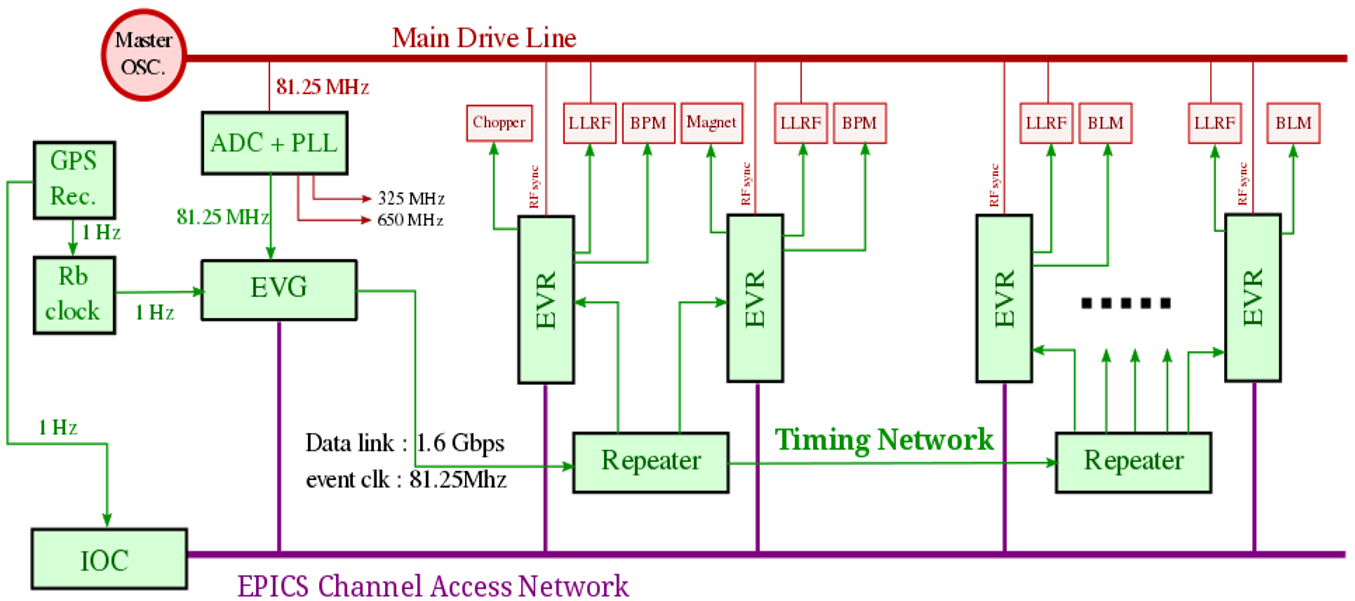
\includegraphics[width=1\columnwidth]{./images/Timing_network.eps}
  %\caption{Overall architecture of the RAON control system}
  \label{fig:architecture}
\end{figure}

\begin{itemize}
\item GPS receiver synchronizes with RB clock and EVG to 1PPS
\item Master OSC. generates reference RF (81.25 MHz) to EVG
\item Two signals of EVG are synchronized by locking phase
\item Synchronized signal of EVG is generated and distributed to EVR according to event code of MRFIOC2 on VME system
\end{itemize}
\end{mdframed}

\columnbreak

\section*{Application using Timing Signal}
%\subsection*{Fast Stepper Motor Control Testbed}
\begin{mdframed}[roundcorner=10pt]
	\begin{figure}[H]
		\centering
		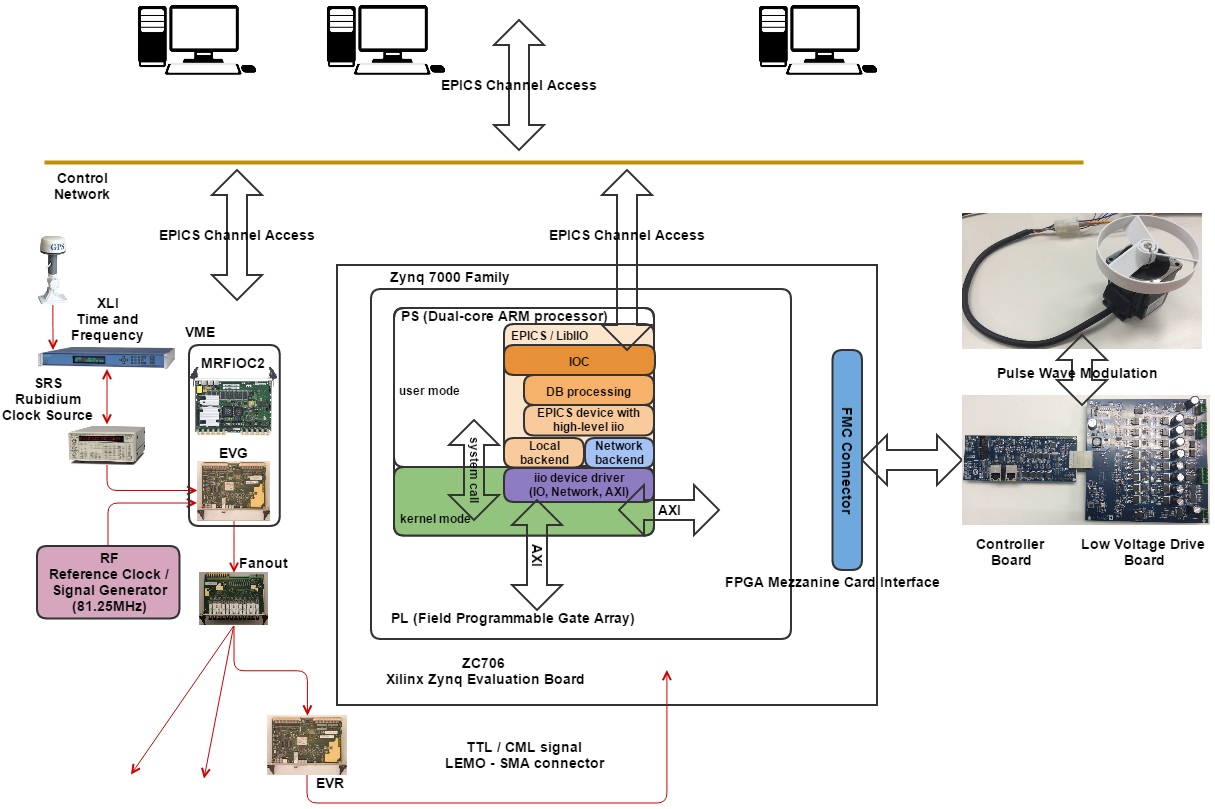
\includegraphics[width=1\textwidth]{./images/WEPGF124f3.eps}
	\end{figure}
%\end{mdframed}
%\begin{mdframed}[roundcorner=10pt]
\begin{itemize}
\item Timing system requires :
  \begin{itemize}
  \item[-] low latency, jitter in fs level.
  \item[-] deterministic operation.
  \item[-] high speed signal processing.
  \item[-] identifying a bunch.
%for RF phase and machine control, and low level RF feedback.
\end{itemize}
\item We will use :
  \begin{itemize}
  \item[-] MRF EVG/EVR hardwares~\cite{MRF}
  \item[-] Libera BPM products~\cite{LIBERABPM}
  \end{itemize}

\item We are considering to :
  \begin{itemize}
  \item[-] use White Rabit for timing system \cite{WR}.
  \item[-] develope homemade BPM with domestic company.
  \end{itemize}
\end{itemize}
\end{mdframed}


\subsection*{Controller / Low Voltage Drive Board for Driving Motor}
\begin{mdframed}[roundcorner=10pt]
\begin{figure}[H]
\centering
  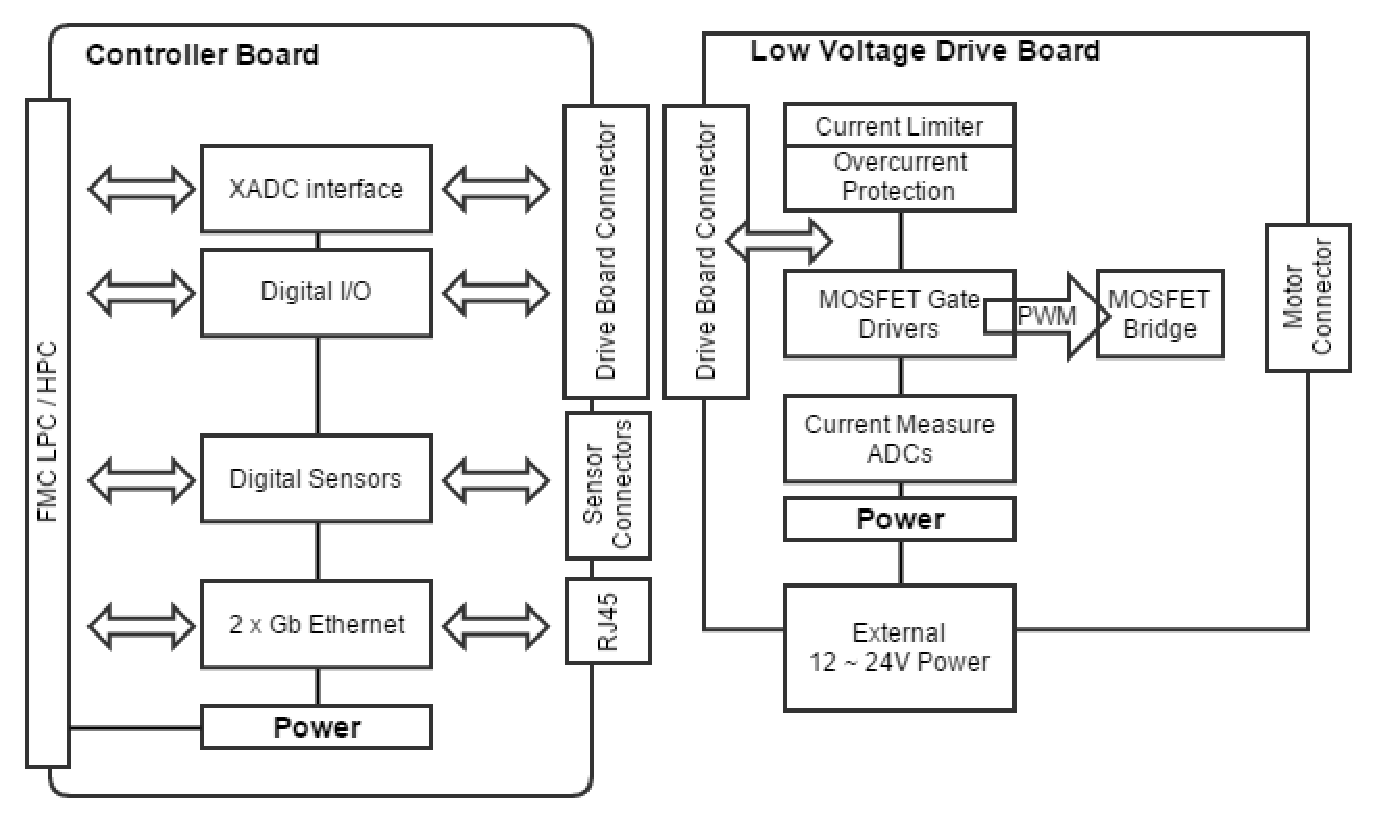
\includegraphics[width=.9\columnwidth]{./images/WEPGF124f2.eps}
%\caption{The timing system prototyping}
\label{fig:timing_prototype}
\end{figure}
\begin{itemize}
\item Two test VME crates consisting of EVG, EVR, and MVME6100 with VxWorks 6.9.
\item Connected via EPICS channel access using fiber cables for event network.
\item Test : jitter, delay time, latency.
\item It will be used to test injector and superconducting LINAC system.
\item The international bidding for prototyping is under way in parallel.
\end{itemize}
\end{mdframed}



\subsection*{The vacuum control system}

\begin{mdframed}[roundcorner=10pt]
\begin{itemize}
\item A testbed for the vacuum control system is being developed with a domestic company.
\item The vacuum system controlled by PLC will be integrated with EPICS and be used for the test facilities.
\end{itemize}
\end{mdframed}

\subsection*{Naming convention}
\begin{mdframed}[roundcorner=10pt]
\begin{itemize}
\item Important for the system integration
\item Should be comprehensive to user and maintainer.
\end{itemize}
%The naming convention is important for the system integration with EPICS,
%because it is related not only to the user comprehension but also
%to the issues on network and hardware I/O and data management.
A primitive naming convention study is done and shown as following:
%and the structure is followed by EPICS style~\cite{esstechnote0005}.
\begin{displaymath}
\textrm{DDDDIII-SSSS:TTTT.XXXX},
\end{displaymath}
where DDDDIII is a device identifier, SSSS is a system name, TTTT is the signal name
followed by the EPICS DB convention, and XXXX is the signal suffix.
This naming convention is not fixed but being improved upon the user's request.
\end{mdframed}



\section*{Conclusion}
\begin{mdframed}[roundcorner=10pt]
Timing system can distribute the fine synchronized event signal at a high speed. The objective of the stepper motor control testbed is to know how to operate the timing system and how to apply it to the high speed controller. The overall implementation is still underway, however if the distributed control system using EPICS makes a connection with the high speed parallel processing of FPGA, it is possible to improve the performance and efficiency of the control system. Zynq SoC can be considered as an ideal device to implement this high-speed control system.
\end{mdframed}

\section*{Acknowledgement}
This work is supported by the Rare Isotope Science Project funded by 
Ministry of Science, ICT and Future Planning (MSIP) 
and National Research Foundation (NRF) of KOREA.

\begin{thebibliography}{9}   % Use for  1-9  references
%\begin{thebibliography}{99} % Use for 10-99 references

\bibitem{TSHOO:NIMB} Y.~K.~Kwon, {\it et. al},``Status of Rare Isotope Science Project in Korea'', Few-Body Syst 54, 961-966, (2013).

\bibitem{mrf}
Micro-Research Finland Oy: \texttt{http://www.mrf.fi}%

\bibitem{amba-bus}
Advanced Microcontroller Bus Architecture:\texttt{http://en.wikipedia.org/wiki/Advanced\_Microcontroller\_Bus\_Architecture}%

\bibitem{analog}
Analog Devices website:
\texttt{http://www.analog.com}

\bibitem{xilix}
Xilinx-FPGA website:
\texttt{http://www.xilinx.com}
%	last visit 27 March 2014.\newline \mbox{ }

\bibitem{zynq}
Zynq-Book Document website:
\texttt{http://www.zynqbook.com}

\bibitem{zc706-doc}
ZC706 Evaluation Board Document:
\texttt{http://www.xilinx.com/support/documentation/boards\_and\_kits/zc706/ug954-zc706-eval-boardxc7z045-ap-soc.pdf}%
\bibitem{linaro}
Linaro Document website :
\texttt{https://en.wikipedia.org/wiki/Linaro}

\bibitem{u-boot}
U-Boot Document website :
\texttt{http://www.denx.de/wiki/U-Boot}

\bibitem{vivado}
Xilinx Vivado Document website :
\texttt{http://www.xilinx.com/products/design-tools/vivado.html}

\bibitem{boot-bin}
Boot Image Document website :
\texttt{http://www.wiki.xilinx.com/Prepare+boot+image}

\bibitem{busybox}
Busybox Document website :
\texttt{http://www.busybox.net/}

\bibitem{iio}
Industrial I/O Document website :
\texttt{https://wiki.analog.com/resources/tools-software/linux-software/libiio}

\bibitem{epics}
EPICS website :
\texttt{http://www.aps.anl.gov/epics/}

%\bibitem{XAL}
%J. Galambos, {\it et. al.}, ``SNS Application Programming Environment'', EPAC 2002, Paris, France (2002).

%\bibitem{esstechnote0005}
%G. Trahern, ``ESS Naming Convention'', ESS AD Technical Note.
\end{thebibliography}
\end{multicols}
%\vspace{13mm}

%\begin{minipage}[b]{1\linewidth}

%\section*{RAON Major Operations Modes}
%\vspace{2mm}
%\begin{figure}[H]
 % 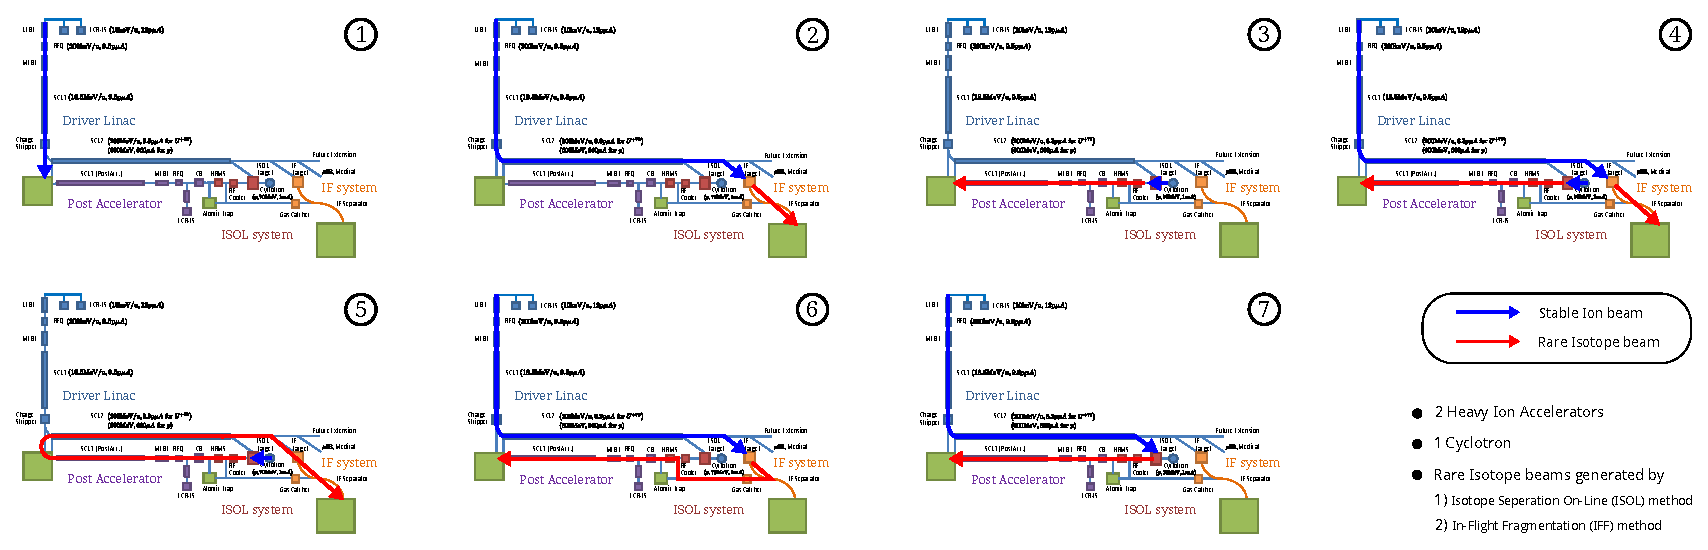
\includegraphics[width=0.99\columnwidth]{./images/raon_all_modes.eps}
%\end{figure}

%\end{minipage}





\end{document}

